% !TEX root = ../thesis.tex

\chapter{Theory}
\label{sec:theory}

% \cleanchapterquote{Users do not care about what is inside the box, as long as the box does what they need done.}{Jef Raskin}{about Human Computer Interfaces}

In this chapter I briefly cover all concepts necessary to fully understand the main contribution of separation of style and content in the field of Neural Networks.
The concepts, after this introduction, will be built bottom-up, meaning that a sequential read should guide the reader logically from question to answer while giving as much insight will be needed to move on and just enough context to understand the raison d'être of the current concept.
The idea is for anybody with basic knowledge in Mathematics and Computing to understand this manuscript from beginning to end.

Having said so, what is an artificial neural network?
That is a very broad question.

\todo[inline]{Polish introduction}
\todo[inline]{Motivations for machine learning}
\todo[inline]{Artificial Neural Networks}
\todo[inline]{Ground Truth??}


% ------------------------------------------------------------------------------

\section{Types of Neural Networks}
\label{sec:Types of Neural Networks}

\begin{description}
  \item[Feed-forward Neural Networks]
  The simplest type of artificial neural network, characterized by its connections not forming cycles and thus the data always flowing in one direction: from input to hidden layers to output.
\end{description}


% ------------------------------------------------------------------------------

\section{Perceptron}
\label{sec:Perceptron}
A perceptron is a type of cell that performs binary classification.

A binary classifier regardless of how it is implemented. It may very well be just a function or a whole deep neural network.

Weight
Also called learnable parameter or just parameter.
Coming from neuroscience literature, it refers to how much importance each one of the different input connections of a neuron has in the activation function.
\todo[inline]

\todo[inline]{Overfitting}

% ------------------------------------------------------------------------------

\section{Multilayer Perceptron}
\label{sec:theory:mlp}
A multilayer perceptron (MLP) is a type of feed-forward neural network composed of several layers where neurons of one layer are fully connected with the next one.
These neural networks are normally used to classify different inputs.

The limitations of the perceptron were mathematically proved \citet{Minsky1969} in 1969 and they claimed perceptrons with multiple layers would not be capable of solving not-linearly separable classes.
Discouraged by these claims little to none research was done in the field of Neural Networks until backpropagation was developed by \citet{Werbos1974}, rediscovered by \citet{Parker1985}, popularized by \citet{Rumelhart1988} and MLP were proved to be universal approximators \cite{Hornik1989,Ruck1990} in 1989.


\subsection{Backpropagation}
\label{sec:theory:mlp:backpropagation}
\todo[inline]


% ------------------------------------------------------------------------------

\section{Convolutional Neural Networks}
\label{sec:theory:convnets}
Convolutional Neural Networks, also known as CNNs or ConvNets, are feed-forward multi-layer neural networks inspired by cats' and monkeys' visual ventral stream \cite{Hubel1968,Lawrence1997} and are responsible for a major breakthroughs in image recognition \cite{LeCun1995}.
Before and contemporaneous to LeCun's LeNet \cite{LeCun1998} other networks like Fukushima's Neocognitron \cite{Fukushima1980} or Riesenhuber \& Poggio's HMAX \cite{Riesenhuber1999} were also inspired in the visual cortex, but it was the former that established the fundamentals for CNNs.
They are able to learn patterns in images from a training set through back-propagation and present built-in resilience towards translation and distortion variances in the input.
Such resilience minimizes pre-processing tasks both for training and classification and greatly reduces human supervision, making CNNs the currently preferred system for image recognition \cite{Visin2015}.

Although multi-layer perceptron are able to perform image recognition, they can only handle images of very small resolution due to the architectural limitations of fully connected layers \cite{ZHANG1999}.
Fully connected layers scale poorly, since neurons of the first hidden layer will process the whole image and will need to store weights for every color channel of every pixel.
Just to give a sense of the scale we are talking, for an RGB image of ${N}\times{M}$ pixels every neuron in a multi-layer perceptron will require storing ${N}\times{M}\times{3}$ weights, which for a ${32}\times{32}$ image it is $3072$ weights, but for a ${1024}\times{1024}$ one is more than $3$ millions.
In the shallower networks, with a single hidden layer, this already implies an exponential memory growth $O(N^2)$ with respect to image resolution.
Not only this is a performance issue in terms of hardware resources, the huge amount of parameters that need to be set also causes the system to quickly overfit.
Worse than that, treating pixels individually as described, regardless of their proximity, does not take into account the spatial information of an image.
That means that to handle variations in the images the network will end up with the same weights being stored in different neurons, proving multi-layer perceptron clearly inefficient for image recognition.
These problems are addressed by CNN architectural features \cite{LeCun1998}: 1) local receptive fields, 2) shared weights, and 3) subsampling.


\subsection{Properties}
\label{sub:concepts:convnets:properties}

\paragraph{Local receptive fields}
The term \emph{receptive field} is borrowed from the literature of neuroscience and it refers to an area of the body surface that trigger a neurological response in the presence of stimuli \cite{Sherrington1906,Alonso2008}.
In the context of convolution networks, receptive field refers to a region of the visual input, represented by an image, that is connected with one or several neurons that will react to it and is commonly called \emph{filter}.
Using local receptive fields means that neurons in the network will not react to the whole image but to a small region of it instead.
This ensures neurons will extract first the most basic visual features such as edges, end-points or corners;
In subsequent layers, from those elementary visual features, neurons will then extract progressively higher-order features like shapes, textures, faces or objects.
Such architecture allows effectively takes into account the spatial correlation existing in images.
Within a layer several neurons performing different feature detections can can be stacked to receive the input from the perceptive field as depicted in Figure~\ref{fig:sec:theory:conv-layer-1}.

\begin{figure}[htb]
  \begin{center}
    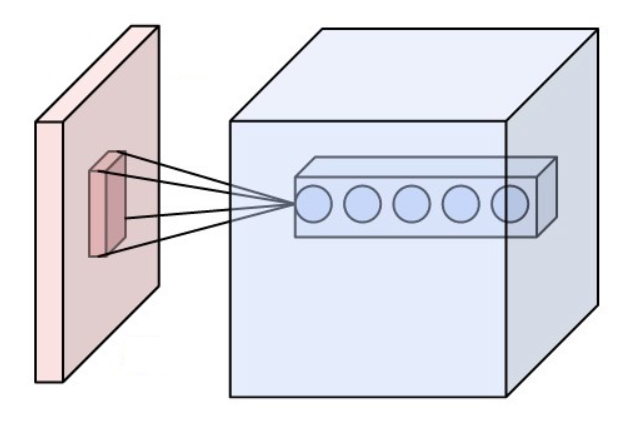
\includegraphics[width=0.6\textwidth]{gfx/conv-layer-1}
  \end{center}
  \caption{Stack of neurons applying different feature detections within a convolutional layer on the same perceptual region \cite{Aphex342015}.}
  \label{fig:sec:theory:conv-layer-1}
\end{figure}

\paragraph{Shared weights}
Layers in CNNs are organized in several slices, each of them containing neurons that detect the same feature but in different regions of the image and each slice detecting different features.
This operation is equivalent to a convolution in image processing, a sliding window that applies a transformation the original image, and that is where CNNs receive their name.
The sliding window is called kernel, filter or mask, and it is an image transformation matrix, usually small, that performs the weighted sum over a set of pixels of the original image, as shown in Figure~\ref{fig:sec:theory:kernel}
In this analogy, the kernel of the convolution is the filter applied by the slice over the input, represented by \emph{weights shared} by all its neurons, being this what makes feature recognition robust against translations or distortions in the image.
The output of the convolution is referred to as \emph{feature map}, and all feature maps produced by a convolutional layer together become the input for the next layer, usually called \emph{volume} since it has height, width and depth.
The height and width are proportional to the size of the original image and depth equal to the amount of slices in the layer.
Such architecture is depicted in Figure~\ref{fig:sec:theory:conv-layer-2}.

\begin{figure}[htb]
  \begin{center}
    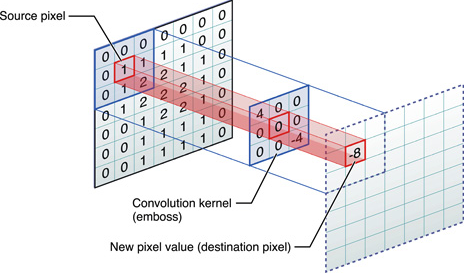
\includegraphics[width=0.5\textwidth]{gfx/kernel}
  \end{center}
  \caption{Convolutional kernel \cite{Apple}. The kernel gets centered on the source pixel and the convolution takes into account nearby pixels transforming the source pixel value. The convolution operation is a weighted sum of the source pixel with its nearby pixels. In this case:\\
    $(0\cdot4)+(0\cdot0)+(0\cdot0)
     +(0\cdot0)+(1\cdot0)+(1\cdot0)
     +(0\cdot0)+(1\cdot0)+(2\cdot-4) = -8$
  }
  \label{fig:sec:theory:kernel}
\end{figure}

\begin{figure}[htb]
  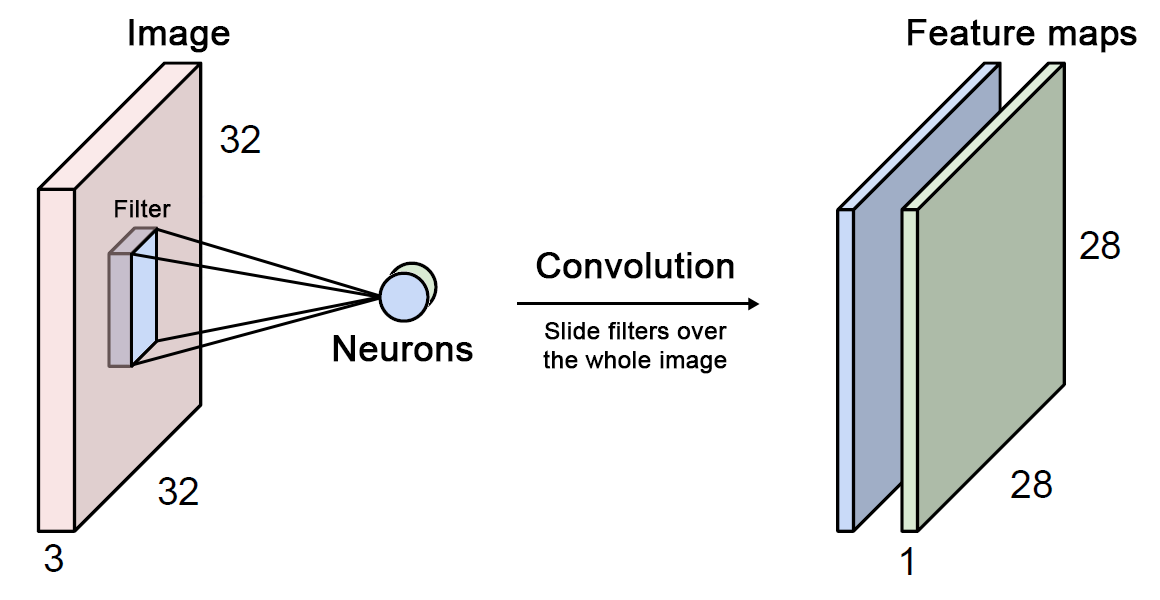
\includegraphics[width=\textwidth]{gfx/conv-layer-2}
  \caption{Anatomy of a convolutional layer and its output \cite{Guerzhoy2016}. On the left there is the representation of an image of ${32}\times{32}$ pixels with $3$ channels (\emph{RGB}). Neurons apply a filter of size ${5}\times{5}\times{3}$ in particular region of the image. Neurons of the same color belong to the same slice apply the same filter in different regions of the image and produce a feature map. All feature maps combined become the "new image" of size ${28}\times{28}\times{N}$, being $N$ the number of slices in the layer, that gets fed to the next layer.}
  \label{fig:sec:theory:conv-layer-2}
\end{figure}

\paragraph{Subsampling}
In the process of detecting higher-order features throughout subsequent layers of the network the exact absolute position of detected features in feature maps is pretty much irrelevant compared to the relative position between them.
For instance, the pattern that describes the number $7$ is an endpoint in upper left area of a horizontal segment, a corner in the upper right area and an endpoint at the bottom of a vertical segment.
Still, small variations in the input may cause the pattern not to be detected because the features will not completely match the filter.
To make the network more robust against variations the sensitivity of the convolutional layers has to be reduced.
This is effectively accomplished by reducing the resolution of the feature maps through non-linear \emph{subsampling} with pooling layers.
$Max$ is normally used as the non-linear function, giving the name of the subsampling operation \emph{max-pooling}, but it is not limited to it, as we will see in Chapter~\ref{sec:system}.
A pooling layer takes as input a volume of feature maps and, usually, has a non-overlapping filter of size ${2}\times{2}$ that gets applied on each one of the feature maps individually, as can be appreciated in Figure~\ref{fig:sec:theory:pooling}.
More specifically, the filter summarizes the feature map by performing max-pooling over its ${2}\times{2}$ regions and producing a single value for each, being this a size reduction of $75\%$.
It is important to note that this reduction applies only to the height and width of the original input since the depth refers to the amount of feature maps and these are preserved.

\begin{figure}
  \begin{subfigure}[b]{0.35\textwidth}
    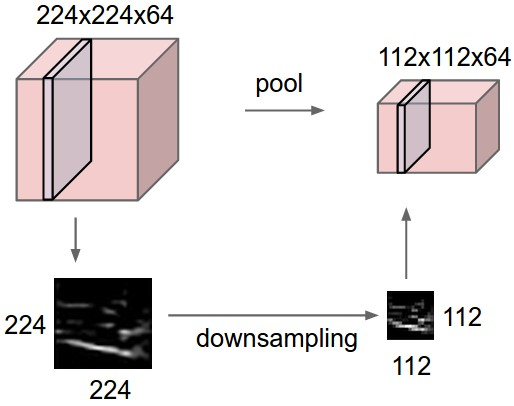
\includegraphics[width=\textwidth]{gfx/pool}
    \captionsetup{justification=centering}
    \caption{General pooling}
    \label{fig:sec:theory:pooling:general}
  \end{subfigure}
  \hfill
  \begin{subfigure}[b]{0.55\textwidth}
    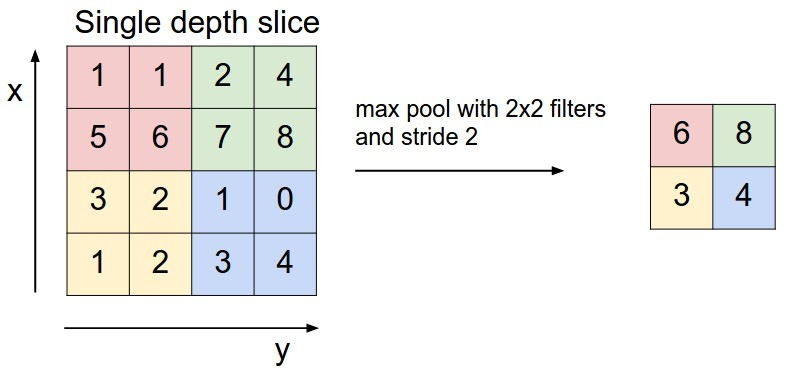
\includegraphics[width=\textwidth]{gfx/maxpool}
    \captionsetup{justification=centering}
    \caption{Max-pooling}
    \label{fig:sec:theory:pooling:max}
  \end{subfigure}
  \caption{Overview of a pooling layer. On the left, the input and output of a pooling layer reducing only the height and width of the volume \cite{Karpathy}. On the right, a single feature map of the input volume being subsampled by non-overlapping ${2}\times{2}$ max-pooling \cite{Karpathya}.}
  \label{fig:sec:theory:pooling}
\end{figure}


\subsection{Architecture}
\label{sub:concepts:convnets:achitecture}

While discussing the properties of ConvNets I have introduced two of their building blocks: convolutional layers and pooling layers.
These alone are not enough to use ConvNets for object recognition tasks since feature extraction is not the same as classification.
Let us have a look at how they fit in the big picture and the rest of the building blocks.

In Figure~\ref{fig:sec:theory:convnet} I present the typical configuration of a complete convolutional network.
We can see convolutional layers are alternated with pooling layers and ultimately fed into a fully connected network.
Whereas convolutional layers typically increase the amount of feature maps increasing the richness of intermediate representations, pooling layers reduce their spatial resolution keeping the amount of parameters low and thus limiting overfitting.
After several convolutional-pooling layers, the set of all feature maps, a highly abstracted representation the original image at that point, gets fed into fully connected layers, usually in the shape of a multilayer perceptron.
It is within the fully connected network that the classification takes place.

\begin{figure}[htb]
  \begin{center}
    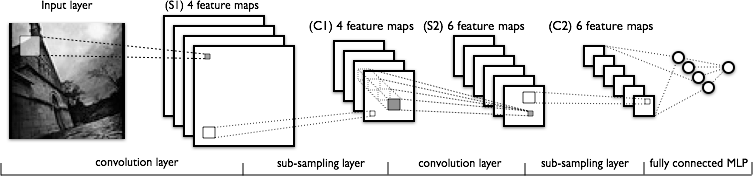
\includegraphics[width=\textwidth]{gfx/conv-network}
  \end{center}
  \caption{LeNet typical architecture \cite{LaboratoiredInformatiquedesSystemesAdaptatifs2010}. On the left there is an image (input layer). The image gets processed by a convolutional layer that extracts 4 elementary features producing 4 feature maps (S1). A pooling layer reduces the dimensionality while maintaining the same amount of feature maps (C1). Next, another convolutional layer extracts 6 higher-order features from the 4 feature maps (C2). Again, another pooling layer reduces the resolution of the 6 feature maps (S2). Finally, a fully-connected network takes the 6 feature maps and performs classification over them.}
  \label{fig:sec:theory:convnet}
\end{figure}

Additionally to these fundamental layers, normalization layers have been used as well.
These, however are \todo{cite}{falling out of use} since their contribution to the final result is close to none and they increase the complexity of the network.
ReLU \cite{Krizhevsky2012,Nair2010}

% It's important to note that all the weights in the network are learnt through back-propagation.

% One last element essential in convolutional networks is the loss layer.
% This layer calculates the error of the classifications


\todo[inline]{TODO}
Summarizing, CNNs are mainly composed by \todo{?}N types of layers: Convolutional layers, pooling layers, ReLU layers, fully connected layers.
Convolutional layers perform feature detection.
Pooling layers reduce the dimensionality of feature maps.
ReLU layers \todo{?}?.
Fully connected layers perform classification.

\paragraph{Feature learning}
Finding kernel that produce the desired feature maps is very difficult since it greatly varies depending on the task.
In CNN, feature learning is the step in which the kernel gets increasingly better at the task of filtering an image or a feature map coming from a previous layer.
\todo[inline]

\subsection{Hyperparameters}
\label{sub:concepts:hyperparameters}

It's worth noting that filters are always applied over the whole depth so that a ${W}\times{H}$ filter


% ------------------------------------------------------------------------------

\section{Convolutional Network Visualization}
\label{sec:theory:netvis}


% ------------------------------------------------------------------------------

\section{Adversarial Networks}
\label{sec:theory:adversarialnet}


% ------------------------------------------------------------------------------

\section{Non-linear transformations}
\label{sec:Non-linear transformations}

They are filters (a.k.a. kernel or feature map), often represented by $\phi$, implemented as functions whose output is not linear to its input often used for feature extraction on images (edges, connectivity, etc.). Perceptron neurons use these as activation function because the dimensionality of the input can be reduced so that it becomes binary classifiable.

\begin{description}
  \item[tanh]
  \item[ReLU]
\end{description}
